%%%%%%%%%%%%%%%%%%%%%%%%%%%%%%%%%%%%%%%%%%%%%%%%%%%%%%%%%%%%
%%% ME301 PROJECT TEMPLATE
%%%%%%%%%%%%%%%%%%%%%%%%%%%%%%%%%%%%%%%%%%%%%%%%%%%%%%%%%%%%


%%%%%%%%%%%%%%%%%%%%%%%%%%%%%%%%%%%%%%%%%%%%%%%%%%%%%%%%%%%%
%%% PREAMBLE
%%%%%%%%%%%%%%%%%%%%%%%%%%%%%%%%%%%%%%%%%%%%%%%%%%%%%%%%%%%%

% Declare document class
\documentclass{AEM4602Wreport}

\usepackage{siunitx}[=v2] % For SI units
\usepackage{rotating}   % For rotating specific elements
\usepackage{textgreek}  % Greek symbols
\usepackage{gensymb}    % Symbols
\usepackage[misc]{ifsym} % For the \Letter symbol
\usepackage{listings}   % For inserting code chunks
\usepackage{colortbl}   % For Knitr table colouring
\usepackage{tabularx}   % For making Knitr tables compatible
\usepackage{longtable}  % For multi-page tables
\usepackage{subcaption}
\usepackage{multirow}
\usepackage{snotez}     % For sidenote environments. enotez for endnotes
\usepackage{csquotes}   % For language-based quote rules (helps BiBLaTeX)
\usepackage{cleveref}   % for clever references 

\usepackage{pifont}
\usepackage{xspace}
\newcommand{\dos}{$\textcolor{leman}{\checkmark}$\xspace}
\newcommand{\donts}{\textcolor{epflred}{\ding{55}}\xspace}
\newcommand{\kindex}[2]{\ensuremath{{#1}_{\scalebox{0.65}{#2}}}}
\newcommand{\U}{\textrm{U}}
\newcommand{\Uinf}{\kindex{\U}{$\infty$}}

%%%%%%%%%%%%%%%%%%%%%%%%%%%%%%%%%%%%%%%%%%%%%%%%%%%%%%%%%%%%
%%% BIBLIOGRAPHY
%%%%%%%%%%%%%%%%%%%%%%%%%%%%%%%%%%%%%%%%%%%%%%%%%%%%%%%%%%%%
\usepackage[		% use biblatex for bibliography
backend=biber,      % use biber or bibtex backend
style=authoryear,   % choose style
natbib=true,		% allow natbib commands
hyperref=true,	    % activate hyperref support
alldates=year,      % only show year (not month)
]{biblatex}

% enter the name of your bibliography file.
% you can create a bib file using a reference managing tool such as Zotero or Mendeley
\addbibresource{sample.bib}

%%%%%%%%%%%%%%%%%%%%%%%%%%%%%%%%%%%%%%%%%%%%%%%%%%%%%%%%%%%%
%%% ARTICLE SETUP
%%%%%%%%%%%%%%%%%%%%%%%%%%%%%%%%%%%%%%%%%%%%%%%%%%%%%%%%%%%%

% Paper title
\title{AEM 4602W Lab Report} % do not change

% Group number:
\groupnumber{4B} % enter your group number

% Authors
% replace by your names, keep the format LAST NAME, First name
\author[1]{LAST NAME, First name}
%\author[4]{LAST NAME, First name}

% keep next line as is
\affil[1]{Department of Aerospace Engineering \& Mechanics, University of Minnesota} % necessary to display all authors

% Email addresses
\correspondence{email.address@umn.edu}


% enter the citation code for your selected paper
\thepaper{\fullcite{ourselectedpaper}}

%%%%%%%%%%%%%%%%%%%%%%%%%%%%%%%%%%%%%%%%%%%%%%%%%%%%%%%%%%%%
%%% ARTICLE START
%%%%%%%%%%%%%%%%%%%%%%%%%%%%%%%%%%%%%%%%%%%%%%%%%%%%%%%%%%%%

% tell us where the figures are 
\graphicspath{{./figurematter/}}

\begin{document}
\maketitle

%%%%%%%%%%%%%%%%%%%%%%%%%%%%%%%%%%%%%%%%%%%%%%%%%%%%%%%%%%%%
\begin{abstract}
Write here the abstract of your report in maximum $200$ words.
Start with one or two sentences that provide a basic motivation for the experiment you designed.
Then, one or two sentences about the experimental setup.
A few sentences about the quantities your measured and the measurement techniques you applied.
One or two sentences about the main challenges and results.
A few sentences summarising the experience.
\end{abstract}

%%%%%%%%%%%%%%%%%%%%%%%%%%%%%%%%%%%%%%%%%%%%%%%%%%%%%%%%%%%%
\section{Introduction}
Briefly describe the application that motivated your experiment.
Then, give a brief sneak peek of what is coming in the rest of the report. 

\section{Materials \& methods}
Carefully present your experimental set-up. 
Describe in detail which quantities you measured and how you measured them. 
Discuss the measurement techniques used and motivate your choice for these techniques. 
Indicate which parameters you varied and how you varied them. 
Do not forget to address the accuracy and resolution of your measurements. 
Do not copy-paste from the course notes, but describe how you adapted the methods to your specific needs.

Based on what you write in this section, anyone should be able to recreate your setup and repeat your measurements. 
\textbf{Repeatability and reproducibility are key to ensuring the validity and reliability of experimental data.}



\subsection{Some general advice}
Introduce every abbreviation and symbol before using it.
\begin{itemize}
\item[\dos] We measured the two-dimensional velocity field $\vec{v}=(u,v)$ using particle image velocimetry (PIV).
\item[\donts] We measured the two-dimensional velocity field $\vec{v}=(u,v)$ using PIV (particle image velocimetry).
\item[\donts] We measured the two-dimensional velocity field $\vec{v}=(u,v)$ Particle Image Velocimetry (PIV).
\end{itemize}

In general, avoid talking in terms of abbreviations.
Suppress the urge to define new wonderful abbreviations (NWA), and do not force your readers to remember your NWA.
You have enough space to write your new wonderful abbreviations out.

If you defined a new important quantity (NIQ) whose values you want to plot later on in a graph, use a symbol to refer to it instead of an abbreviation.
For example, assume you determined some characteristic maximum velocity, introduce a symbol with a subscript that is intuitive like $\kindex{v}{max}$ and use this symbol in your plots.
Examples of less intuitive or confusing symbols would be $\pi$, $\kindex{v}{3}$, $\kindex{q}{m}$, ...
Continue to write about this characteristic maximum velocity in the text instead of writing about $\kindex{v}{max}$ as much as you can.

As a writer, you want something from your readership.
You want to communicate your message, let others know what you learned, and get the satisfaction of people understanding and appreciating your work and using it or building upon it.
That means that \textbf{you} have to do the work.
You must make it as easy as possible for the reader to follow your story.
Assume that your readers are lazy, and do not force them to memorise your nomenclature or abbreviation.
Do not be afraid of repetitions or parallelism in writing.
Your reader will appreciate it!

\subsection{Another subsection}
You can never have just one subsection.
You can have no subsections or at least two.
That makes sense, right?
After all, a list with only one item is not a list.

\begin{figure}[b!] % use only b or t not h
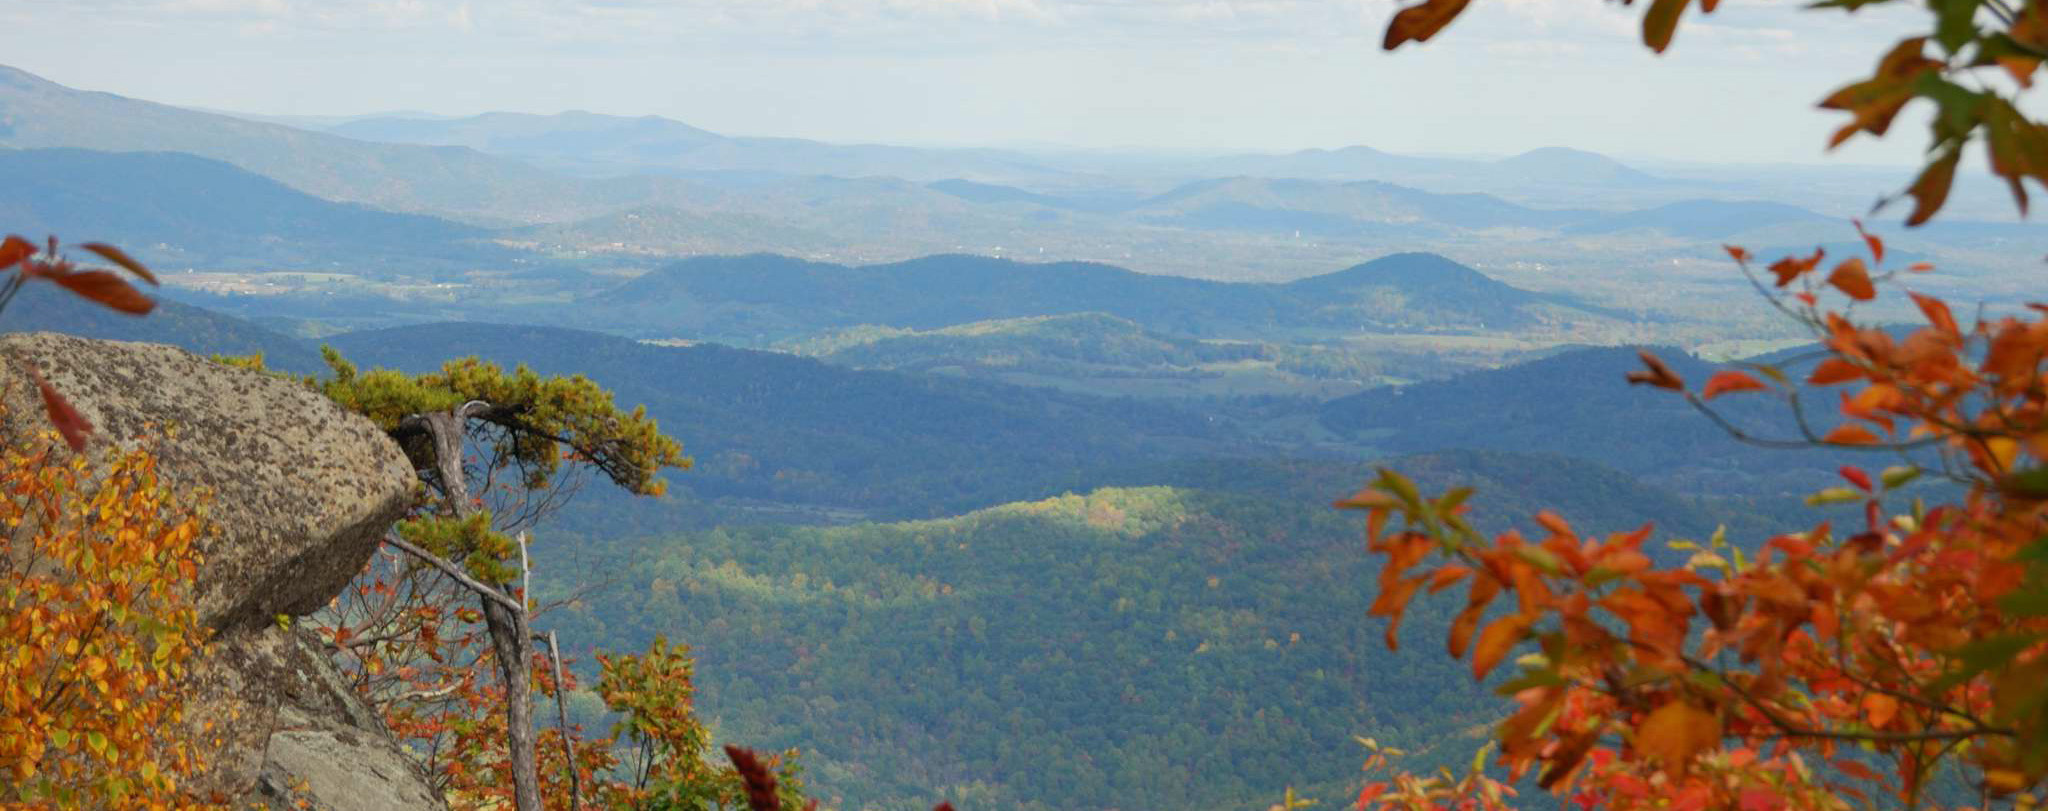
\includegraphics[width=\textwidth]{view}
\caption{A wide figure that takes up the entire text width.}
\label{fig:view}
\end{figure}

\section{Results}
Present your results clearly and concisely.
Discuss the accuracy and the resolution of your data. 
Address unexpected results and potential sources of error and provide recommendations or ideas for improvement.

Please pay special attention to how you present your results visually. 
Technical information becomes easier to understand when supported by a visual element. 
Good visuals already explain half the story.
A good figure, like a good text, needs work and iterations. 
You can find \textit{ten simple rules for better figures} by \cite{betterfigures}.

\begin{figure}[tb!]
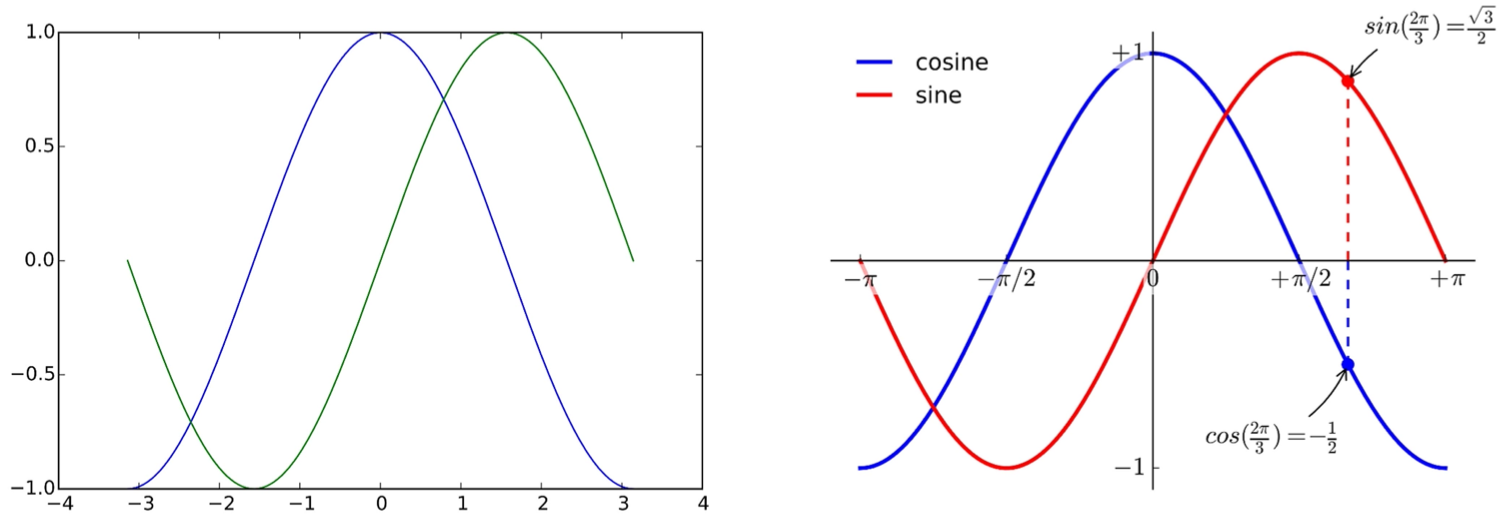
\includegraphics[width=\textwidth]{badgood}
\caption{Example figure from \cite{betterfigures} to prove that you should not trust the defaults. The left panel shows the sine and cosine functions rendered by matplotlib using default settings. The right panel is visually improved by tweaking various settings. 
The axes should have axes labels. 
}
\label{fig:results}
\end{figure}

\subsection{Some advice}
Less is often more.
You do not need to show all the data you generated or analysed during your project, but you do need to describe and discuss in detail all the data and all figures that your show.
Be selective in the data and figures that you show.
The figures should support the arguments that you are trying to make.

%\lipsum[1-1]

%\begin{table}[b!]
%    \caption{Example of a table.}\label{tab:table}
%    \begin{tabular}{l c r} % <-- Alignments: 1st column left, 2nd middle and 3rd right, with vertical lines in between
%    \toprule
%    \textbf{Value 1} & \textbf{Value 2} & \textbf{Value 3}\\
%    \midrule
%    1 & 11.1 & a\\
%    3 & 23.1 & c\\
%    \bottomrule
%    \end{tabular}
%\end{table}

When building up a story, start with setting the scene before you jump into the details.
Your readers are not necessarily familiar with your experiment.
Be kind to them and guide them through your report.
Your report should not be a puzzle the reader is trying to solve.
It is your job to feed them the information in a logical order.


\subsection{Some more advice}
All figures should be presented in the order in which they are discussed in the text.
So, you first discuss the view presented in \cref{fig:view}.
Then, you make the argument that is supported by the data in \cref{fig:results}.
The \verb+\cref{label}+ command from the \textit{cleveref} package automatically determines the type of item (equation, figure, etc.) you are referring to.
\Cref{tab:table} presents a rather useless table.
Tables are often not the most intuitive way to present information, so only use them if there is really no better alternative.
Note that we used \verb+\Cref{label}+ here to start the sentence with a capital letter.

\section{Conclusion}
Summarise your work and results.
Start by repeating what the motivation for the experiment was, briefly recapitulate what you did, and then summarise the main findings.
If possible, add how these results are relevant in the bigger picture and what their impact is.

\subsection{Author contributions}
Briefly summarise the contributions of the different group members.

\subsection{Acknowledgement}
Optional - your acknowledgements for your pets, friends, and family.

\printbibliography

%%%%%%%%%%%%%%%%%%%%%%%%%%%%%%%%%%%%%%%%%%%%%%%%%%%%%%%%%%%%
%%% SUPPLEMENTARY MATERIAL / APPENDICES
%%%%%%%%%%%%%%%%%%%%%%%%%%%%%%%%%%%%%%%%%%%%%%%%%%%%%%%%%%%%
%% Note the different way of including figures in the appendix.


%%%%%%%%%%%%%%%%%%%%%%%%%%%%%%%%%%%%%%%%%%%%%%%%%%%%%%%%%%%%
%%% ARTICLE END
%%%%%%%%%%%%%%%%%%%%%%%%%%%%%%%%%%%%%%%%%%%%%%%%%%%%%%%%%%%%

\end{document}

